\documentclass[11pt,a4paper]{article}
\usepackage[T1]{fontenc}
\usepackage[margin=2.3cm]{geometry}
\usepackage{amsmath,amssymb}
\usepackage{graphicx}
\usepackage[dvipsnames]{xcolor}
\usepackage{enumitem}
\usepackage[colorlinks=true,linkcolor=blue,urlcolor=blue]{hyperref}
\setlength{\parskip}{0.6em}
\setlength{\parindent}{0pt}
\begin{document}

\begin{center}{\LARGE\bfseries openstereodic}\\[0.4em]{\large Measure how a stretched surface deforms in 3D, using only two cameras and random dots.}\\[0.2em]\small PAN IIT OSS explainer \textbullet{} higher secondary to advanced undergraduate (levels 4-6)\end{center}

\section*{Why this exists}
Stereo digital image correlation measures the shape and the deformation of a loaded surface with two cameras and a random dot pattern. This explainer shows the mathematics behind it: the pinhole camera, triangulation, matching patches to a fraction of a pixel, and turning displacements into strain.

\section*{The end goal}
Measure 3D surface strain from two cameras (stereo digital image correlation). The end goal is a 3D surface strain map from two cameras, as used in materials testing laboratories for rubbers, metals and biological tissue. The same ideas drive photogrammetry, robot vision and motion capture.

\section*{How the three sessions build up}
\begin{enumerate}[nosep]
\item \textbf{Session 1: A camera flattens the world; two cameras recover depth} (Level 1, conceptual interactive model, 60 min).
\item \textbf{Session 2: From matched pixels to millimetres: triangulation and sub-pixel matching} (Level 2, mathematical engineering model, 75 min).
\item \textbf{Session 3: Digital image correlation on speckle images, validated} (Level 3, simulation and validation, 90 min).
\end{enumerate}

\section{Session 1: A camera flattens the world; two cameras recover depth}

\subsection*{A. Real-world problem}
Close one eye, hold a finger at arm's length and switch eyes: the finger jumps against the background, much more than the wall behind it does. A single photograph cannot tell you how far things are, but two photographs taken a few centimetres apart can. Labs use exactly this to measure the shape of a loaded rubber strip without touching it. How is a 3D position found from two flat pictures?

\subsection*{B. Concept and theory}
A pinhole camera lets light from a point (X, Y, Z) pass through a tiny hole and land on a sensor a distance f behind it. By similar triangles the landing place is u = f X / Z sideways and v = f Y / Z upward. We count f in pixels, so u and v are in pixels from the middle of the image. Put camera 2 a distance B (the baseline) to the right of camera 1, both looking straight ahead. For camera 2 the point is B closer to the left, so u2 = f (X - B) / Z. The sideways jump d = u1 - u2 (the disparity) is f B / Z: it contains no X, only the depth Z. Turn it around and Z = f B / d.

\begin{itemize}[nosep]
\item X, Y, Z: position of the point: sideways, up, distance in front of camera 1 (m)
\item f: focal length measured in pixels (px)
\item B: baseline: distance between the two cameras (m)
\item u1, u2: sideways image coordinate in camera 1 and 2, from the image centre (px)
\item d: disparity u1 - u2 (px)
\end{itemize}

\begin{equation*}
u=\frac{fX}{Z},\qquad v=\frac{fY}{Z}
\end{equation*}

\begin{equation*}
u_1=\frac{fX}{Z},\qquad u_2=\frac{f(X-B)}{Z}
\end{equation*}

\begin{equation*}
d=u_1-u_2=\frac{fB}{Z}\quad\Longleftrightarrow\quad Z=\frac{fB}{d}
\end{equation*}

\begin{center}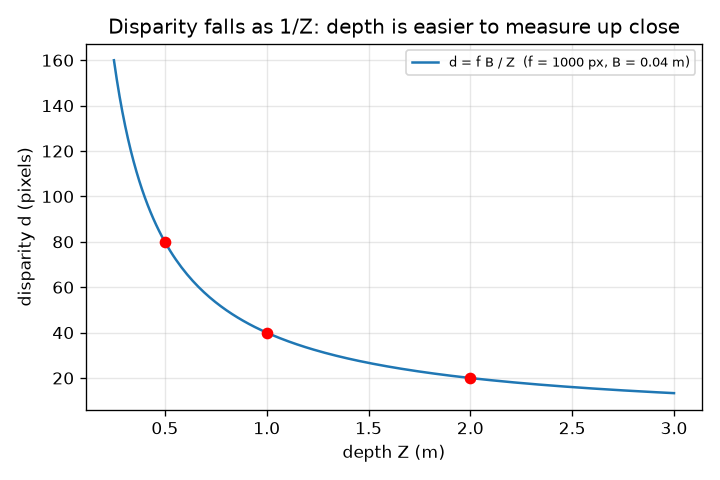
\includegraphics[width=0.85\linewidth]{figures/s01_disparity_vs_depth.png}\\\small Disparity against depth: the 1 / Z curve for f = 1000 px and B = 0.04 m.\end{center}

\subsection*{E. Worked example}
With f = 1000 px and B = 0.04 m, a point sits at X = 0.02 m, Y = 0.01 m, Z = 0.5 m. Where does each camera see it, what is the disparity, and does Z = f B / d give back 0.5 m?
\begin{enumerate}[nosep]
\item Camera 1: u1 = 1000 * 0.02 / 0.5 = 40 px and v = 1000 * 0.01 / 0.5 = 20 px.
\item Camera 2: u2 = 1000 * (0.02 - 0.04) / 0.5 = -40 px (the point is left of its centre line), v = 20 px.
\item Disparity d = u1 - u2 = 40 - (-40) = 80 px. Check with f B / Z = 1000 * 0.04 / 0.5 = 80 px.
\item Depth back from the disparity: Z = f B / d = 1000 * 0.04 / 80 = 0.5 m.
\end{enumerate}
\textbf{Answer.} Camera 1 sees (40, 20) px, camera 2 sees (-40, 20) px, the disparity is 80 px and the depth is recovered as 0.5 m.

\subsection*{F. Questions}
\begin{enumerate}[nosep]
\item \textbf{Conceptual.} Why does the disparity not depend on the sideways position X of the point?
\item \textbf{Numerical.} Two cameras 0.06 m apart with f = 1000 px measure a disparity of 25 px. How far away is the point? Is the answer sensible?
\item \textbf{Graph and simulation interpretation.} In the graph of disparity against depth, what happens to the disparity when the depth is doubled from 0.5 m to 1.0 m, and what does that mean for the accuracy?
\item \textbf{Design and optimisation challenge.} Design: with f = 1000 px, choose a baseline so that one pixel of disparity corresponds to at most 5 mm of depth at 0.5 m. What is the cost of a longer baseline?
\end{enumerate}

\section{Session 2: From matched pixels to millimetres: triangulation and sub-pixel matching}

\subsection*{A. Real-world problem}
Session 1 said Z = f B / d, but a real camera gives pixels, and the computer must find the matching spot in the second picture by comparing small patches of random dots (speckle). If the match can only be found to a whole pixel, a surface 0.5 m away is located only to about 3 mm, which is useless for seeing a rubber strip stretch. How well can matching be done, and how does a matching error turn into a depth error?

\subsection*{B. Concept and theory}
A calibrated pair means f, B and the principal point (the image centre, CX, CY) are known. A matched pair (uL, vL) in the left image and uR in the right image gives d = uL - uR, Z = f B / d, X = (uL - CX) Z / f and Y = (vL - CY) Z / f. A small error dd in the disparity gives to first order dZ = (Z\textasciicircum{}2 / (f B)) dd, so depth error grows with the square of the distance and shrinks with a longer baseline. To find the match, take a patch (a subset) of 2h + 1 pixels from the left row and slide it along the right row; at each slide k compute the zero-normalised cross-correlation C(k), which is 1 for a perfect match even if brightness and contrast differ. The best whole-pixel slide k0 is where C peaks. Fitting a parabola through C(k0 - 1), C(k0), C(k0 + 1) gives the sub-pixel peak. The true hill is not exactly a parabola, so the estimate is pulled slightly (pixel locking); for random dots of size sigma the hill is close to exp(-D\textasciicircum{}2 / (4 sigma\textasciicircum{}2)), which predicts the bias.

\begin{itemize}[nosep]
\item uL, vL, uR: pixel coordinates of the matched point in the left and right images (px)
\item CX, CY: principal point (image centre), 160 and 80 (px)
\item dd: error of the measured disparity (px)
\item dZ: resulting depth error (m)
\item C(k): zero-normalised cross-correlation at trial shift k (no unit)
\item h: subset half-size; the subset is 2h + 1 pixels wide (px)
\item sigma: size of one speckle dot (Gaussian standard deviation) (px)
\end{itemize}

\begin{equation*}
d=u_L-u_R,\quad Z=\frac{fB}{d},\quad X=\frac{(u_L-C_X)Z}{f},\quad Y=\frac{(v_L-C_Y)Z}{f}
\end{equation*}

\begin{equation*}
\delta Z\approx\frac{fB}{d^{2}}\,\delta d=\frac{Z^{2}}{fB}\,\delta d
\end{equation*}

\begin{equation*}
C(k)=\frac{\sum (f_i-\bar f)(g_{i+k}-\bar g)}{\sqrt{\sum (f_i-\bar f)^2\,\sum (g_{i+k}-\bar g)^2}}
\end{equation*}

\begin{equation*}
k^{*}=k_0+\frac{C(k_0-1)-C(k_0+1)}{2\,\big[C(k_0-1)-2C(k_0)+C(k_0+1)\big]}
\end{equation*}

\begin{center}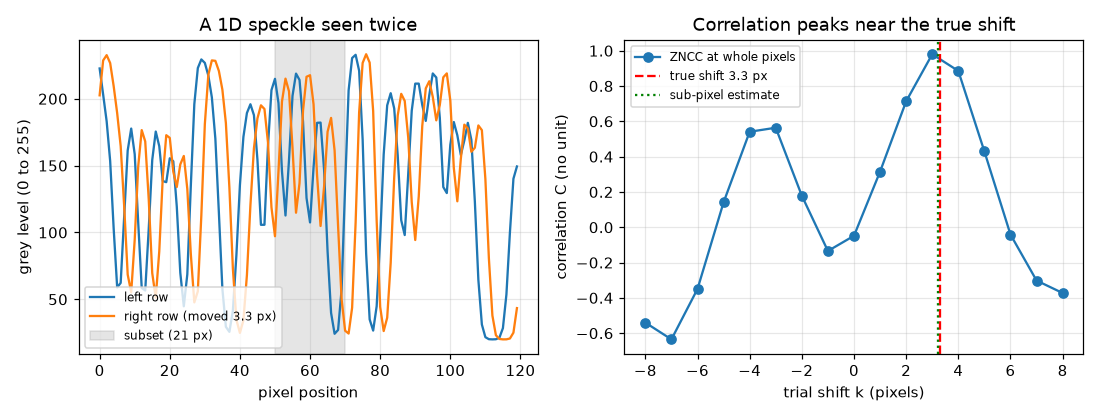
\includegraphics[width=0.85\linewidth]{figures/s02_correlation_peak.png}\\\small A 1D speckle seen twice (shift 3.3 px) and the correlation of a 21-pixel subset: peak at 3, sub-pixel estimate 3.24.\end{center}

\subsection*{E. Worked example}
With f = 1000 px, B = 0.04 m and principal point (160, 80): a matched pair is uL = 200, vL = 100, uR = 120. Find the 3D point. If the disparity is uncertain by 0.05 px, what is the depth uncertainty?
\begin{enumerate}[nosep]
\item Disparity d = 200 - 120 = 80 px.
\item Z = f B / d = 1000 * 0.04 / 80 = 0.5 m.
\item X = (200 - 160) * 0.5 / 1000 = 0.02 m and Y = (100 - 80) * 0.5 / 1000 = 0.01 m.
\item Depth error dZ = Z\textasciicircum{}2 dd / (f B) = 0.25 * 0.05 / 40 = 0.0003125 m = 0.3125 mm.
\item For comparison, whole-pixel matching (dd = 0.5 px) gives 3.125 mm.
\end{enumerate}
\textbf{Answer.} The point is (0.02, 0.01, 0.5) m; a 0.05 px disparity error gives 0.31 mm of depth error, ten times better than whole-pixel matching.

\subsection*{F. Questions}
\begin{enumerate}[nosep]
\item \textbf{Conceptual.} Why do we match patches of random dots rather than single pixels, and what goes wrong on a blank patch?
\item \textbf{Numerical.} At Z = 1.2 m with f = 1000 px and B = 0.04 m, what depth error comes from a disparity error of 0.1 px?
\item \textbf{Graph and simulation interpretation.} In the sub-pixel bias graph, at which fractional shifts is the error zero, and why is it largest in between?
\item \textbf{Design and optimisation challenge.} Design: choose a baseline so that the depth error at 0.5 m is at most 0.2 mm when sub-pixel matching gives dd = 0.05 px. What changes if matching is only good to 0.1 px?
\end{enumerate}

\section{Session 3: Digital image correlation on speckle images, validated}

\subsection*{A. Real-world problem}
A rubber strip is painted with random dots and pulled. Two photographs, before and after, are all we have. Where did each patch of dots move, and how much was the rubber stretched? Digital image correlation (DIC) answers both by matching small square subsets between the images. Because we make the images ourselves from a known deformation, we can grade the method: how close does it get, and what limits it?

\subsection*{B. Concept and theory}
The reference image shows a point X at pixel (x, y); after loading the same material point is at x + u(X). DIC finds u by taking a subset of (2h+1) x (2h+1) pixels around (x0, y0) and searching the deformed image for the best match, scored by zero-normalised sum of squared differences. A whole-pixel search gives a start; Gauss-Newton steps refine six numbers: the displacement (u, v) and the four gradients (u,x, u,y, v,x, v,y), which let the subset stretch and shear (an affine shape function). Grey levels between pixels come from cubic convolution interpolation. Strain is the slope of the displacement field, e\_xx = du/dx and e\_yy = dv/dy (small strain), taken from a least-squares plane fitted to a window of (2w+1)\textasciicircum{}2 grid points to limit noise. For image noise of sigma\_n grey levels in each image and a mean squared image gradient G2, the random displacement error of one subset is sigma\_u = sqrt(2) sigma\_n / sqrt(N G2) with N = (2h+1)\textasciicircum{}2. If displacement curves like b x\textasciicircum{}2, a subset that can only shift and stretch picks up a bias of about b h (h + 1) / 3 pixels, so there is an optimum subset size. The synthetic test uses u = a (x - xc) + b (x - xc)\textasciicircum{}2 and v = -nu a (y - yc) with a = 0.02, b = 1e-4 per pixel and nu = 0.45.

\begin{itemize}[nosep]
\item u, v: displacement of a subset centre in x and y (px)
\item h: subset half-size (the subset is 2h+1 wide) (px)
\item a, b: strain and curvature of the test displacement field (no unit, 1/px)
\item nu: Poisson ratio (sideways contraction per stretch) (no unit)
\item sigma\_n: camera noise in each image (grey levels)
\item G2: mean squared image gradient in x ((grey/px)\textasciicircum{}2)
\item w: strain window half-size in grid points (no unit)
\item e\_xx, e\_yy: strain in x and in y (no unit)
\end{itemize}

\begin{equation*}
u=a(x-x_c)+b(x-x_c)^2,\qquad v=-\nu a(y-y_c)
\end{equation*}

\begin{equation*}
\varepsilon_{xx}=\frac{\partial u}{\partial x}=a+2b(x-x_c),\qquad \varepsilon_{yy}=\frac{\partial v}{\partial y}=-\nu a
\end{equation*}

\begin{equation*}
\sigma_u=\frac{\sqrt{2}\,\sigma_n}{\sqrt{(2h+1)^2\,G_2}}
\end{equation*}

\begin{equation*}
\text{bias}\approx\frac{b\,h(h+1)}{3},\qquad \sigma_\varepsilon=\frac{\sigma_u}{\Delta\,(2w+1)\sqrt{w(w+1)/3}}
\end{equation*}

\begin{center}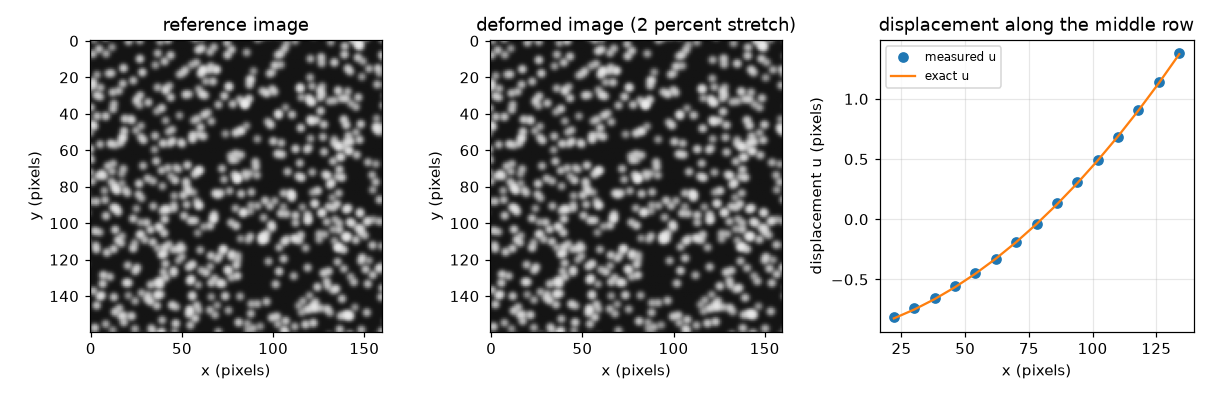
\includegraphics[width=0.85\linewidth]{figures/s03_dic_images.png}\\\small Reference and deformed speckle images, and the measured displacement against the exact curve along the middle row.\end{center}

\subsection*{E. Worked example}
For u = 0.02 (x - 80) + 1e-4 (x - 80)\textasciicircum{}2 find u at x = 56 and x = 104, the strain at x = 80 from these two points, and the random displacement error for noise 4 grey levels, h = 10 and G2 = 471.
\begin{enumerate}[nosep]
\item u(56) = 0.02 * (-24) + 1e-4 * 576 = -0.48 + 0.0576 = -0.4224 px.
\item u(104) = 0.02 * 24 + 1e-4 * 576 = 0.48 + 0.0576 = 0.5376 px.
\item Strain = (0.5376 - (-0.4224)) / (104 - 56) = 0.96 / 48 = 0.0200. The curvature terms are equal at both points and cancel, so this equals the exact strain a = 0.02 at x = 80.
\item Subset size N = (2 * 10 + 1)\textasciicircum{}2 = 441 pixels, so sigma\_u = sqrt(2) * 4 / sqrt(441 * 471) = 5.657 / 455.8 = 0.0124 px.
\item Measured noise-only error in the code: 0.0118 px, within 5 percent of the prediction.
\end{enumerate}
\textbf{Answer.} u(56) = -0.4224 px, u(104) = 0.5376 px, strain 0.0200; the predicted noise error is 0.0124 px.

\subsection*{F. Questions}
\begin{enumerate}[nosep]
\item \textbf{Conceptual.} Why is the speckle pattern random and high-contrast, and why can the image change brightness without hurting the match?
\item \textbf{Numerical.} For noise 6 grey levels, subset half-size h = 14 and G2 = 471, find the random displacement error, and the strain error from noise for a window half-size w = 2 with grid spacing 8 px.
\item \textbf{Graph and simulation interpretation.} In the plot of displacement error against subset size, why does each curve have a minimum, and what moves it?
\item \textbf{Design and optimisation challenge.} Design: with noise 6 grey levels and G2 = 471, choose the smallest strain window (w = 1, 2 or 3, grid spacing 8 px, h = 14) so the strain error from noise stays below 0.001. What do you lose with a larger window?
\end{enumerate}

\section{Real-world mini-project}
\textbf{Measure the strain of a stretched rubber strip from two stereo pairs.} A lab photographs a rubber strip before and after loading with two parallel cameras. Both pairs come from \texttt{stereo\_pair} in Session 3: the unloaded pair is \texttt{stereo\_pair(strip\_dots(), 0.0, 0.0, noise=3.0, seed=10)} and the loaded pair is \texttt{stereo\_pair(strip\_dots(), 0.03, 0.010, noise=3.0, seed=20)}. You are not told what happened to the strip. Use \texttt{track\_subset} (Session 3) and your own triangulation (Session 2, with the principal point at the image centre (160, 80); the strip appears about 80 px further left in the right image) to find: the depth of the strip before and after, and its strain in x. Then repeat the strain calculation with the left images only, as a single-camera analysis would.

\section{The path ahead}
\begin{enumerate}[nosep]
\item \textbf{Session 4: Second-order shape function.} A matching function with a quadratic shape function (12 parameters) and a test on a strongly curved field.
\item \textbf{Session 5: Large motion and seed propagation.} A tracker that follows a whole grid through displacements far larger than the search window.
\item \textbf{Session 6: Calibrate the stereo rig.} A calibration routine and a reprojection-error report.
\item \textbf{Session 7: 3D strain on a curved surface.} A stereo pipeline that reconstructs a bulging specimen and reports the strain along it.
\item \textbf{Session 8: A load history.} An animation of the measured strain map over 30 load steps.
\end{enumerate}

\section{Answers and hints}

\subsection*{Session 1}
\begin{enumerate}[nosep]
\item \textbf{Conceptual.} Hint: Write u1 - u2 and see what happens to the terms that contain X. Solution: u1 = f X / Z and u2 = f (X - B) / Z, so u1 - u2 = f X / Z - f X / Z + f B / Z = f B / Z. The X terms cancel. Both cameras see the point shifted sideways by the same amount f X / Z; only the baseline term f B / Z remains, and that depends on the depth.
\item \textbf{Numerical.} Hint: Z = f B / d. Check the units: px * m / px = m. Solution: Z = 1000 * 0.06 / 25 = 2.4 m. Sanity check: a larger disparity means nearer, and 25 px is smaller than the 60 px we would get at 1 m, so a point beyond 1 m is consistent. Units: px * m / px = m.
\item \textbf{Graph and simulation interpretation.} Hint: Read the values at 0.5 m, 1 m and 2 m. Solution: The disparity halves each time the depth doubles: 80 px at 0.5 m, 40 px at 1 m, 20 px at 2 m (the 1 / Z shape). The curve is steeper close up, so one pixel of disparity error corresponds to 6.2 mm of depth at 0.5 m but 95 mm at 2 m. The same matching accuracy gives much worse depth far away.
\item \textbf{Design and optimisation challenge.} Hint: Use depth step = Z squared / (f B + Z) for a one pixel change, and solve for B. Solution: We need 0.25 / (1000 B + 0.5) \textless{}= 0.005, so 1000 B + 0.5 \textgreater{}= 50 and B \textgreater{}= 0.0495 m. A baseline of 0.05 m gives a step of 4.95 mm and a disparity of 100 px at 0.5 m. The cost: with cameras further apart each sees the object from a more different angle, so the two pictures overlap less, matching gets harder (a bigger search range and more perspective change), and the rig is bulkier. Assumption: parallel cameras and exact f.
\end{enumerate}

\subsection*{Session 2}
\begin{enumerate}[nosep]
\item \textbf{Conceptual.} Hint: Think about how many places in the other image look like one pixel, and what correlation does with a constant patch. Solution: A single pixel value looks like thousands of others; a patch of random dots is almost unique, so its correlation peaks sharply at one place. On a blank (constant) patch every pixel equals the mean, the denominator of the correlation is zero and there is nothing to match, which the code reports as correlation 0 instead of guessing. That is why specimens are painted with a random, high-contrast pattern.
\item \textbf{Numerical.} Hint: dZ = Z\textasciicircum{}2 dd / (f B). Solution: dZ = 1.44 * 0.1 / 40 = 0.0036 m = 3.6 mm. Sanity check: at 0.5 m the same 0.1 px gives 0.625 mm, and 1.2 m is 2.4 times further, so the error should be 2.4\textasciicircum{}2 = 5.76 times bigger: 0.625 * 5.76 = 3.6 mm.
\item \textbf{Graph and simulation interpretation.} Hint: Look at where the three samples are symmetric around the peak. Solution: The error is zero at 0 and 0.5. At 0 the peak sits exactly on a sample and the neighbours are symmetric; at 0.5 the peak is exactly between two samples, which is again symmetric about the answer. In between the three samples are lopsided and the parabola, which is not the true hill shape, is pulled toward the nearest whole pixel; the measured pull is about 0.01 to 0.02 px near 0.3 and 0.7 (opposite signs).
\item \textbf{Design and optimisation challenge.} Hint: B = Z\textasciicircum{}2 dd / (f dZ). Solution: B = 0.25 * 0.05 / (1000 * 0.0002) = 0.0625 m = 62.5 mm. The disparity at 0.5 m is then 125 px, so the search range must be wider and the overlap of the two views smaller. With dd = 0.1 px the baseline doubles to 125 mm, which is hard to build for a small field of view, so improving the matching (better speckle, less noise) is cheaper than moving the cameras apart. Trade-off: baseline versus overlap and matching difficulty.
\end{enumerate}

\subsection*{Session 3}
\begin{enumerate}[nosep]
\item \textbf{Conceptual.} Hint: Think about uniqueness of a patch, and what subtracting the mean and dividing by the spread does. Solution: A random pattern makes every patch unique, so the correlation has one sharp peak; a regular pattern would match at many places, and a smooth one has no gradient to lock onto (the Gauss-Newton matrix becomes singular, and the code returns NaN for a blank patch). Contrast gives a large image gradient G2, which lowers the noise error as 1 / sqrt(G2). Subtracting each patch's mean and dividing by its spread removes brightness offsets and contrast scaling, so only the pattern's shape is compared.
\item \textbf{Numerical.} Hint: sigma\_u = sqrt(2) sigma\_n / sqrt(N G2), N = 29\textasciicircum{}2; then divide by 8 (2w+1) sqrt(w (w+1) / 3). Solution: N = 841, N * G2 = 396111, sqrt = 629.4. sigma\_u = 1.4142 * 6 / 629.4 = 0.0135 px. Strain: 8 * 5 * sqrt(2) = 56.57, so sigma\_e = 0.0135 / 56.57 = 0.00024. Sanity check: 0.0135 px over a 40 px baseline is 3e-4, the same order. The real error is about 30 percent bigger because neighbouring subsets overlap.
\item \textbf{Graph and simulation interpretation.} Hint: Which term dominates for small subsets, and which for large ones? Solution: For small subsets there are few pixels, so noise dominates and the error falls like 1 / (2h+1). For large subsets the subset cannot follow the curved displacement, and the bias b h (h + 1) / 3 grows like h\textasciicircum{}2. The two cross at the minimum, near h = 14 to 19 for both noise levels in the figure. More noise moves the optimum to larger subsets (the noise curve is higher); more curvature moves it to smaller ones (the bias curve is higher).
\item \textbf{Design and optimisation challenge.} Hint: Use sigma\_e = sigma\_u / (8 (2w+1) sqrt(w (w+1) / 3)) with sigma\_u = 0.0135 px. Solution: w = 1: 8 * 3 * sqrt(2/3) = 19.6, so sigma\_e = 0.0135 / 19.6 = 0.00069 (below 0.001; allowing 30 percent extra for overlap gives about 0.0009, still passing, but with little margin). w = 2 gives 0.00024 with a lot of margin. Choose w = 1 for the best spatial resolution (the window spans 2 * 8 + 29 = 45 px) or w = 2 for safety (61 px). The cost of a bigger window is spatial resolution: a sharp strain peak (such as a neck) is smoothed and its height underestimated.
\end{enumerate}

\section{How to join}
Read \texttt{CONTRIBUTING.md} in the repository, then pick an issue labelled \texttt{good first issue}. Repository: \url{https://github.com/KrunalPanchal1995/openstereodic}

\end{document}
